% This is "sig-alternate.tex" V2.0 May 2012
% This file should be compiled with V2.5 of "sig-alternate.cls" May 2012
%
% This example file demonstrates the use of the 'sig-alternate.cls'
% V2.5 LaTeX2e document class file. It is for those submitting
% articles to ACM Conference Proceedings WHO DO NOT WISH TO
% STRICTLY ADHERE TO THE SIGS (PUBS-BOARD-ENDORSED) STYLE.
% The 'sig-alternate.cls' file will produce a similar-looking,
% albeit, 'tighter' paper resulting in, invariably, fewer pages.
%
% ----------------------------------------------------------------------------------------------------------------
% This .tex file (and associated .cls V2.5) produces:
%       1) The Permission Statement
%       2) The Conference (location) Info information
%       3) The Copyright Line with ACM data
%       4) NO page numbers
%
% as against the acm_proc_article-sp.cls file which
% DOES NOT produce 1) thru' 3) above.
%
% Using 'sig-alternate.cls' you have control, however, from within
% the source .tex file, over both the CopyrightYear
% (defaulted to 200X) and the ACM Copyright Data
% (defaulted to X-XXXXX-XX-X/XX/XX).
% e.g.
% \CopyrightYear{2007} will cause 2007 to appear in the copyright line.
% \crdata{0-12345-67-8/90/12} will cause 0-12345-67-8/90/12 to appear in the copyright line.
%
% ---------------------------------------------------------------------------------------------------------------
% This .tex source is an example which *does* use
% the .bib file (from which the .bbl file % is produced).
% REMEMBER HOWEVER: After having produced the .bbl file,
% and prior to final submission, you *NEED* to 'insert'
% your .bbl file into your source .tex file so as to provide
% ONE 'self-contained' source file.
%
% ================= IF YOU HAVE QUESTIONS =======================
% Questions regarding the SIGS styles, SIGS policies and
% procedures, Conferences etc. should be sent to
% Adrienne Griscti (griscti@acm.org)
%
% Technical questions _only_ to
% Gerald Murray (murray@hq.acm.org)
% ===============================================================
%
% For tracking purposes - this is V2.0 - May 2012

\documentclass{sig-alternate}


\begin{document}
%
% --- Author Metadata here ---
\conferenceinfo{WOODSTOCK}{'97 El Paso, Texas USA}
%\CopyrightYear{2007} % Allows default copyright year (20XX) to be over-ridden - IF NEED BE.
%\crdata{0-12345-67-8/90/01}  % Allows default copyright data (0-89791-88-6/97/05) to be over-ridden - IF NEED BE.
% --- End of Author Metadata ---

\title{Counting Features\titlenote{(Produces the permission block, and
copyright information). For use with
SIG-ALTERNATE.CLS. Supported by ACM.}}


%
% You need the command \numberofauthors to handle the 'placement
% and alignment' of the authors beneath the title.
%
% For aesthetic reasons, we recommend 'three authors at a time'
% i.e. three 'name/affiliation blocks' be placed beneath the title.
%
% NOTE: You are NOT restricted in how many 'rows' of
% "name/affiliations" may appear. We just ask that you restrict
% the number of 'columns' to three.
%
% Because of the available 'opening page real-estate'
% we ask you to refrain from putting more than six authors
% (two rows with three columns) beneath the article title.
% More than six makes the first-page appear very cluttered indeed.
%
% Use the \alignauthor commands to handle the names
% and affiliations for an 'aesthetic maximum' of six authors.
% Add names, affiliations, addresses for
% the seventh etc. author(s) as the argument for the
% \additionalauthors command.
% These 'additional authors' will be output/set for you
% without further effort on your part as the last section in
% the body of your article BEFORE References or any Appendices.

\numberofauthors{3} %  in this sample file, there are a *total*
% of EIGHT authors. SIX appear on the 'first-page' (for formatting
% reasons) and the remaining two appear in the \additionalauthors section.
%
\author{
% You can go ahead and credit any number of authors here,
% e.g. one 'row of three' or two rows (consisting of one row of three
% and a second row of one, two or three).
%
% The command \alignauthor (no curly braces needed) should
% precede each author name, affiliation/snail-mail address and
% e-mail address. Additionally, tag each line of
% affiliation/address with \affaddr, and tag the
% e-mail address with \email.
%
% 1st. author
Xinyang Gao
}
% There's nothing stopping you putting the seventh, eighth, etc.
% author on the opening page (as the 'third row') but we ask,
% for aesthetic reasons that you place these 'additional authors'
% in the \additional authors block, viz.

\date{\today}
% Just remember to make sure that the TOTAL number of authors
% is the number that will appear on the first page PLUS the
% number that will appear in the \additionalauthors section.

\maketitle
\begin{abstract}
In CTR estimation problems for online advertising, the feature engineering work is a crucial part. For example, Baidu extracts hundreds of billions of binary features (or called model features) to train a huge linear regression estimator. On the other side, there is another kind of features, called counting features, which are always continuous and normally only have less than 1000 in number in CTR estimation tasks. For a simple example, consider the user city feature. For the binary model features, if there are 10k cities in the dataset, there should be 10k unique binary features, of which only one has the value 1 while others are all valued as 0 (referred as one-hot encoding). For counting features, there are only two for the city description no matter how many cities there are in the dataset: (i) the average CTR given the city (e.g., 0.12\% for Shanghai); (ii) the frequency of such city in the dataset (e.g., 10 million).

Generally, model features are widely used in linear regression based estimators such as logistic regression. Counting features are used in the tree models such as random forest or gradient boosting regression tree for their continuity property. However, there is no work extensively studying the comparison and relationship of these two kinds of features. Particularly, the literature on counting feature based CTR estimation is very rare.

This work aims at giving an extensive study on the counting feature based CTR estimators and their comparison against model features based ones. Perhaps we could also find other good counting features for the CTR estimator modelling, not just the average value and frequency.


\end{abstract}

% A category with the (minimum) three required fields
\category{H.4}{Information Systems Applications}{Miscellaneous}
%A category including the fourth, optional field follows...
\category{D.2.8}{Software Engineering}{Metrics}[complexity measures, performance measures]

\terms{Theory}

\keywords{}

\section{Introduction}
In this paper, the following aspects will be discussed:

\begin{itemize}
\item The performance of counting feature is comparable to binary feature
\item The counting feature can be used to solve the cold start problem to some extent
\item A generalized model can be built for cold start problem
\end{itemize}

\section{CTR Prediction and Current Challenges}

\subsection{CTR Prediction Based on Linear Model}
\subsection{CTR Prediction Based on Non-linear Model}
\subsection{Cold-start:How to apply prediction model on New Advertisement Campaign}

\section{Feature Engineering}
\subsection{Introduction of Counting Feature}
\subsection{Relation Between Counting Feature and Binary Feature Based on Linear Model}
\subsubsection{Frequency Feature}
\setlength{\parindent}{5ex}

The \textsl{Click Through Rate} (CTR) prediction problem can be characterized as a logistic regression problem. we can use features of ads, terms, and advertisers to learn a model that accurately predicts the CTR for new ads. To train the prediction model, we firstly define the following symbols for later explanations.\vspace{5mm}
The training dataset contains number of \textsl{N} instances, which are the records in datalog containing \textsl{M} fields of user, advertiser and publisher information, as well as their clicking information for each ad impression. The result of the impression, namely whether the user clicks on the ad will be represent by \textsl{y}. Even though normally we use logistic regression to train the model since the dependent variable is dichotomous, here the liner regression is used to prove the relation between model built by \(x_{\text{counting}}\) representing the data instances encoded into \textsl{Counting Feature} and model built by \(x_{\text{binary}}\) representing the data instances encoded into one-hot \textsl{Binary Feature}. The dimension of \(x_{\text{counting}}\) is the number of fields \textsl{M} well the dimension of \(x_{\text{binary}}\) is represend by \textsl{D} for which \(D >> M\). The more detailed information about symbols are shown as follows:
\begin{itemize}
\item  Binary Features : \(x_{\text{binary}(N\times D)}\)
\item  Counting Feature : \(x_{\text{counting}(N\times D)}\)
\item  Clicking result : \(y_{(1\times N)}\)
\item  Weights vector of Binary Feature : \(w_{\text{binary}(1\times D)}\)
\item  Weights vector of Counting Feature: \(w_{\text{counting}(1\times M)}\)
\item  Transform Binary Feature to Counting Feature matrix : \(T_{(M\times D)}\)
\item  Calculating feaquency matrix : \(A_{(N\times 1)}\) which is an all-one vector 
$\vec{1 }$  
\item  Field  matrix : \(C_{(M\times D)}\) which is a 0-1 matrix concatenated with \textsl{}{M} vectors \(V_{m,(m = 1...M)}\) and in each vector \(V_m\) only its corresponding positions in field \textsl{m} is filled with 1, with other positions 0.
\item  Diag function : Transform the column vector into a diagonal matrix.\vspace{5mm} 

\end{itemize}
 It can be proven that 
\[ T = C\times Diag(x_{binary}A) \]
The formation of \textsl{T} is 

$$
\begin{pmatrix} 
\vec{F_1} \\
\vec{F_2} \\
.\\
\vec{F_M}

\end{pmatrix}
$$

\noindent in which \($$\vec{F_m}$$ = $$\begin{pmatrix} 
$$\vec{0 }$$ , f_{m1}, f_{m2}, ...f_{mi}... , f_{mI} ,$$\vec{0 }$$ 
\end{pmatrix}$$\), and \(f_{mi}\) represents the occurrence of \(i_{th}\) binary feature in the field \textsl{m} in the whole dataset.\vspace{5mm}

\noindent Next, the relations between \(w_{\text{binary}}\) and \(w_{\text{counting}}\) are proven as follows. 

\begin{equation}
w_{\text{binary}} \times x_{\text{binary}}^T = y 
\end{equation}

\begin{equation}
(w_{\text{binary}}^T \times w_{\text{binary}}) \times x_{\text{binary}}^T = w_{\text{binary}}^T \times y 
\end{equation}

\begin{equation}
x_{\text{binary}}^T = (w_{\text{binary}}^T \times w_{\text{binary}})^{-1} \times w_{\text{binary}}^T \times y 
\end{equation}

Using SVD, we can derive that,

\begin{equation}
(w_{\text{binary}}^T \times w_{\text{binary}})^{-1} \times w_{\text{binary}}^T = (w_{\text{binary}})^{-1(left)}  
\end{equation}

So we can get that 
\begin{equation}
x_{\text{binary}}^T =  (w_{\text{binary}})^{-1(left)} \times y 
\end{equation}

We define
\begin{equation}
T = C \times Diag(x_{\text{binary}}^T \times A)
\end{equation}


Multiply each size by \textsl{T}, we can get
 
\begin{equation}
T \times x_{\text{binary}}^T =  T \times (w_{\text{binary}})^{-1(left)} \times y 
\end{equation}

It can be proven that 
\begin{equation}
T \times x_{\text{binary}}^T =  x_{\text{counting}}
\end{equation}

So
\begin{equation}
x_{\text{counting}} =  T \times (w_{\text{binary}})^{-1(left)} \times y 
\end{equation}

Since \(T \times (w_{\text{binary}})^{-1(left)}\) is a \(M \times 1\) matrix, so multiplying its transposition we can get a constant scalar, 
\begin{equation}
(T \times (w_{\text{binary}})^{-1(left)})^T \times (T \times (w_{\text{binary}})^{-1(left)}) = \lambda
\end{equation}

So, 
\begin{equation}
1/{\lambda} \times (T \times (w_{\text{binary}})^{-1(left)})^T \times x_{\text{counting}} =  y
\end{equation}

In conclusion, we can get
\begin{equation} \label{eq:12}
\begin{split}
w_{\text{counting}} & =\ 1/{\lambda} \times (T \times (w_{\text{binary}})^{-1(left)})^T \\
& = \ 1/{\lambda} \times (C \times Diag(x_{\text{binary}}^T \times A) \times (w_{\text{binary}})^{-1(left)})^T
\end{split}
\end{equation}

\subsubsection{Average CTR feature}

\setlength{\parindent}{5ex}

In this section, the relation between  \(w_{\text{ctr}}\) and \(w_{\text{binary}}\) will be deduced, the steps are similar except for specific part of CTR calculating. \vspace{3mm}

Initially, we can get the similar deduction process, 
\begin{equation}
w_{\text{binary}} \times x_{\text{binary}}^T = y 
\end{equation}

\begin{equation}
(w_{\text{binary}}^T \times w_{\text{binary}}) \times x_{\text{binary}}^T = w_{\text{binary}}^T \times y 
\end{equation}

\begin{equation}
x_{\text{binary}}^T = (w_{\text{binary}}^T \times w_{\text{binary}})^{-1} \times w_{\text{binary}}^T \times y 
\end{equation}

\begin{equation}
(w_{\text{binary}}^T \times w_{\text{binary}})^{-1} \times w_{\text{binary}}^T = (w_{\text{binary}})^{-1(left)}  
\end{equation}

\begin{equation}
x_{\text{binary}}^T =  (w_{\text{binary}})^{-1(left)} \times y 
\end{equation}

However, then in order to count the number of \textsl{clicks} for each instance, we redefine the transformation matrix \textsl{T} as following, 

\begin{equation}
T_{\text{click}} = C \times Diag(x_{\text{binary}}^T \times y)
\end{equation}



From section 1, we can know that, 
\begin{equation}
T_{\text{frequency}} = C \times Diag(x_{\text{binary}}^T \times A)
\end{equation}

Since it is easy to know that,

\begin{equation}
(Diag(T_{\text{click}}) \times (1/T_{\text{frequency}} )^T =  T_{\text{ctr}}
\end{equation}

Similar to section 1, we can multiply \(T_{\text{ctr}}\) by both sides of equation (17)

\begin{equation}
T_{\text{ctr}} \times x_{\text{binary}}^T =  T_{\text{ctr}} \times (w_{\text{binary}})^{-1(left)} \times y 
\end{equation}

It can be proven that 

\begin{equation}
T_{\text{ctr}} \times x_{\text{binary}}^T =  x_{\text{ctr}}
\end{equation}

So,

\begin{equation}
 x_{\text{ctr}} =  T_{\text{ctr}} \times (w_{\text{binary}})^{-1(left)} \times y 
\end{equation}

It is similar to section 1 that \(T_{\text{ctr}} \times (w_{\text{binary}})^{-1(left)}\)is a \(M \times 1\) matrix, so we define, 
\begin{equation}
(T_{\text{ctr}} \times (w_{\text{binary}})^{-1(left)})^T \times (T_{\text{ctr}} \times (w_{\text{binary}})^{-1(left)}) = \lambda
\end{equation}

So, 
\begin{equation}
1/{\lambda} \times (T_{\text{ctr}} \times (w_{\text{binary}})^{-1(left)})^T \times x_{\text{ctr}} =  y
\end{equation}

In conclusion, we can get
\begin{equation} 
\begin{split}
w_{\text{ctr}} & =\ 1/{\lambda} \times (T_{\text{ctr}} \times (w_{\text{binary}})^{-1(left)})^T \\
& = \ 1/{\lambda} \times (Diag(T_{\text{click}}) \times (1/T_{\text{frequency}} )^T \\ 
& \times (w_{\text{binary}})^{-1(left)})^T \\
& = \ 1/{\lambda} \times (Diag(C \times Diag(x_{\text{binary}}^T \times y)) \\ 
& \times (1/ (C \times Diag(x_{\text{binary}}^T \times A) )^T) \times (w_{\text{binary}})^{-1(left)})^T
\end{split}
\end{equation}


From the above parts we can see that the weights of counting feature and counting feature itself satisfy that:
\begin{equation}
w_{\text{counting}} = f(x_{\text{counting}})
\end{equation}
So assuming that for the same dataset if the input binary features follows linear regression model, then the corresponding counting feature will follow non-linear model, so it is reasonable we compare the results of logistic regression of binary feature with that of GBRT model for counting feature, the comparison is as follows:
\subsection{Adform Dataset Introduction and Performance of CTR Prediction with Counting and Binary Feature}


\section{Dataset Bias Anaysis}
\subsection{Bias of Advertisement Campaign Datasets}
\subsection{Domain Adaptation and Transfer Learning}
\subsection{Cross-Dataset Generalization}

\section{Cold Start CTR prediction}
In this part, the cold start problem will be discussed. Now the experiment is done in which the placement id is counted and when the clicks in one palcement id's corresponding is higher than 200, the instances will be remained, and the overlap of placement id in the train dataset and test dataset will be filtered out. Then for the training dataset all the campains in the test dataset are new. Many experiments are done now but result is confused. Generally the result is as follows: 

Performance of Binary Feature in cold start > Counting Feature with update weights using new coming data > Counting feature without update weights using weights from previous campains > Binary feature without update weights


I am trying to figure out the reason why binary feature performs well in cold start problem and it seems biased dataset is a cause and I try to split the model into generic and specific parts and overcome the bias.
\subsection{Model Similarity Analysis}
At first, we will start from the easier one, the frequency feature. Let's assume that we have two datasets, dataset \(Dataset_{\text{1}}\) and \(Dataset_{\text{2}}\), for each dataset we can get \(w_{\text{counting}}\) and \(w_{\text{binary}}\) respectively. Let's abbreviate them as \(w_{\text{c1}}\) and \(w_{\text{b1}}\) as well as \(w_{\text{c2}}\) and \(w_{\text{b2}}\). 

From \ref{eq:12} we can get the following equation:
\begin{equation} \label{eq:28}
\begin{split}
w_{\text{counting}} & =\ 1/{\lambda} \times (C \times Diag(x_{\text{binary}}^T \times A) \times (w_{\text{binary}})^{-1(left)})^T \\
& = \ 1/{\lambda} \times (C \times Diag(x_{\text{binary}}^T \times A) \times ((w_{\text{binary}}^T \times w_{\text{binary}})^{-1} \\
& \times w_{\text{binary}}^T )^T
\end{split}
\end{equation}

We will make use of cos similarity, which is used to measure the distance between two vectors to measure the similarity of two \(w_{\text{counting}}\) from \(Dataset_{\text{1}}\) and \(Dataset_{\text{2}}\). The formation of similarity can be shown as follows:

\begin{equation} \label{29} 
\begin{split}
Similarity & = \cos(\Theta) = \frac{w_{\text{c1}} \times w_{\text{c2}}^T} {||w_{\text{c1}}|| \times ||w_{\text{c2}}|| }
\end{split}
\end{equation}

Substitute \(w_{\text{c1}}\) with \ref{eq:12} and represent \(Diag(x_{\text{binary}}^T \times A)\) using \(Diag(f)\) since this diagonal entries \(d(i,i) \) shows the frequency of feature \(i\), we can get the following equation:


\begin{equation} \label{30} 
\begin{split}
\frac{w_{\text{c1}} \times w_{\text{c2}}^T} {||w_{\text{c1}}|| \times ||w_{\text{c2}}|| } & =  \frac{w_{\text{c1}} \times w_{\text{c2}}^T} {\sqrt{w_{\text{c1}} \times w_{\text{c1}}^T} \times \sqrt{w_{\text{c1}} \times w_{\text{c2}}^T} }
\end{split}
\end{equation}

To simply, at first we will deduct the following equation:

\begin{equation} \label{31} 
\begin{split}
w_{\text{ci}} \times w_{\text{cj}}^T & = \frac{1}{{\lambda}_{i}{\lambda}_{j} } \times (w_{\text{bi}} \times Trans_{i}) \times (w_{\text{bj}} \times Trans_{j})^T \\
& subject : (i.j = 1 \cup 2)
\end{split}
\end{equation}


In which \(Trans\) is a Transformation Matrix, 
\begin{equation} \label{31} 
\begin{split}
Trans = ((w_{\text{binary}}^T \times w_{\text{binary}})^{-1})^T \times (Diag(f))^T \times C^T  
\end{split}
\end{equation}

Then, we will focus on the transformation matrix. 

Since \(((w_{\text{binary}}^T \times w_{\text{binary}})^{-1})^T\) is a symmetric matrix, so it equals to its own transposition. 
\subsection{Minimise Dataset Bias}

\section{Experiment}
The data from 3-14 to 3-27 are regarded as training dataset, the data from 5- are regarded as test dataset, the count of training dataset is, test dataset is 

\begin{table*}[h]
\centering
\begin{tabular}{ |c|c|c|c| } 
\hline
Shared Campaign  & Unique Train Dataset Campaign & Unique Test Dataset Campaign \\
\hline
1310190 & 1307617, 884194, 1283235, 1335301  & 1466432, 1448738 \\ 
& 1385319, 1349577, 1276074, 1363723 & 1406405, 1424966 \\ 
&  1357245, 1341802, 1341937, 1307838 & 1424330, 1445998 \\ 
&  1285558, 1358167, 1305663, 1299899 & 1458704, 1454382 \\
&  1363711, 1386205, 1368830, 1366271 &  1472727, 1452138 \\
\hline
\end{tabular}
\label{tab:campainid}
\end{table}

Only the instances from the campaign with more than 500 clicks and 50000 impressions will be remained, the campaigns can be classified as the ones shared by the training and test dataset, the ones unique to training dataset and the one unique to test dataset.  

\(1/3\) of the training dataset is used as train dataset, \(2/3\) will be used as count dataset. In order to increase the generalization of training dataset to improve the universality of the trained prediction model, four campaign will constitute one training dataset and two campaigns are used to make up a test dataset to decrease the bias of test dataset.  

For the sake of convenience, the training dataset will be labeled as 1,2,3,4 and 5, from top to the bottom, as well as the test dataset. For each training dataset, the prediction model will be build based on it which will be used to test the data stream from each of the test dataset, the result is in 6.3.

\subsection{Experiment Setup - Dataset Preparation}
\subsection{Measurement Methods}
\subsection{Performance of Cold-start CTR prediction using Binary and Counting Feature}

Experiment 1.1: Training Dataset 1 (141366), Test Dataset 1 (243525):
\begin{figure}
\centering
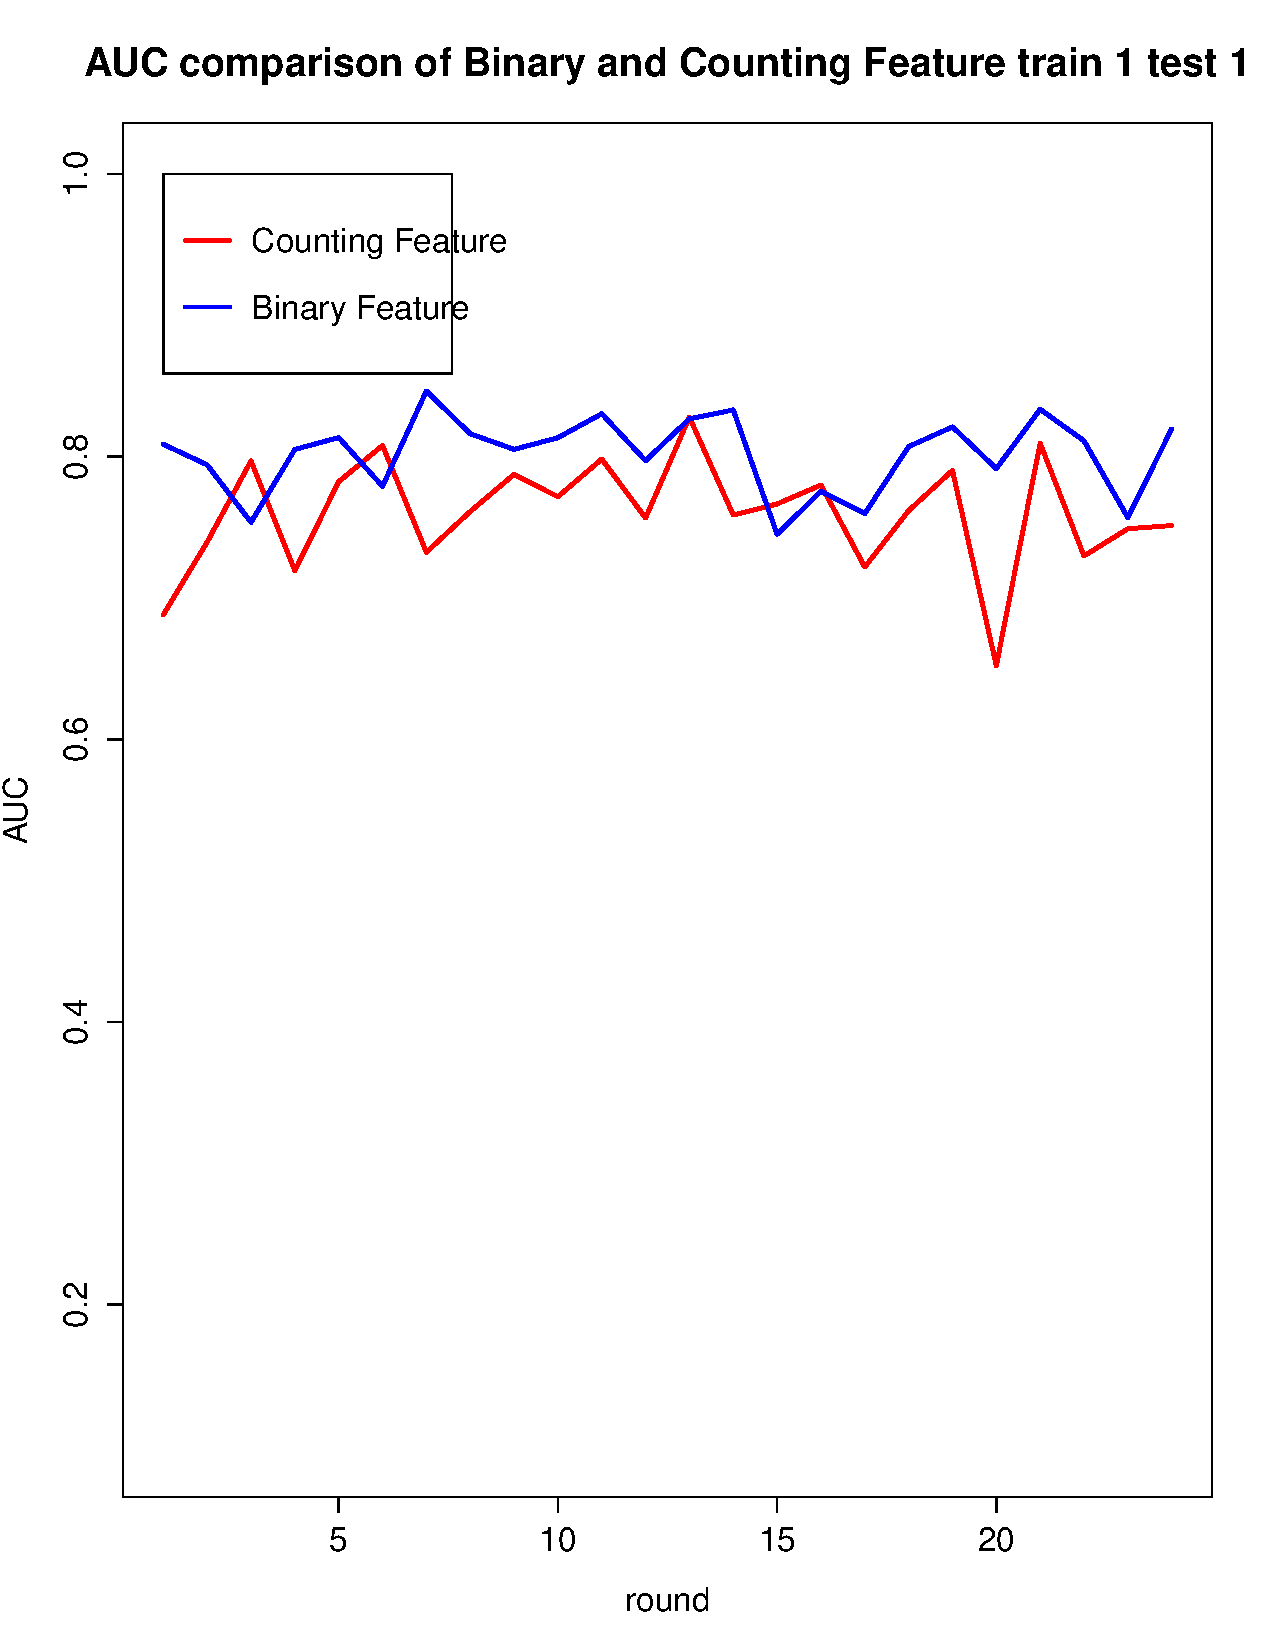
\includegraphics[width=1.\columnwidth]{imagescoldstart/train1test1.pdf}
\caption{Caption}
\label{fig:my_label}
\end{figure}


Experiment 1.2: Training Dataset 1 (141366), Test Dataset 2 (44445):

Experiment 1.3: Training Dataset 1 (141366), Test Dataset 3 (97563):




Experiment 2.1: Training Dataset 2 (90664), Test Dataset 1 (243525):

Experiment 2.2: Training Dataset 2 (90664), Test Dataset 2 (44445):

Experiment 2.3: Training Dataset 2 (90664), Test Dataset 3 (97563):




Experiment 3.1: Training Dataset 3 (14366), Test Dataset 1 (243525):

Experiment 3.2: Training Dataset 3 (141366), Test Dataset 2 (44445):

Experiment 3.3: Training Dataset 3 (141366), Test Dataset 3 (97563):
























\section{Conclusions}

%\end{document}  % This is where a 'short' article might terminate

%ACKNOWLEDGMENTS are optional
\section{Acknowledgments}




%
% The following two commands are all you need in the
% initial runs of your .tex file to
% produce the bibliography for the citations in your paper.
\bibliographystyle{abbrv}
\bibliography{sigproc}  % sigproc.bib is the name of the Bibliography in this case
% You must have a proper ".bib" file
%  and remember to run:
% latex bibtex latex latex
% to resolve all references
%
% ACM needs 'a single self-contained file'!
%
%APPENDICES are optional
%\balancecolumns

\end{document}
